\documentclass[a4paper,10pt]{article}
\usepackage[utf8]{inputenc}
\usepackage{amsmath}
\usepackage{subcaption}
\usepackage{notoccite}
\usepackage{xargs}                      % Use more than one optional parameter in a new commands
\usepackage[pdftex,dvipsnames]{xcolor}  % Coloured text etc.
\usepackage[colorinlistoftodos,prependcaption,textsize=tiny]{todonotes}
% note: disable any of the following commands by adding 'disable' as a first option after \todo
% see example below
\newcommandx{\tobecompleted}[2][1=]{\todo[linecolor=red,backgroundcolor=red!25,
bordercolor=red,#1]{#2}}
\newcommandx{\thiswillnotshow}[2][1=]{\todo[disable,linecolor=OliveGreen,
backgroundcolor=OliveGreen!25,bordercolor=OliveGreen,#1]{#2}}

\DeclareMathOperator*{\argmin}{argmin} 
\DeclareMathOperator*{\argmax}{argmax} 

%opening
\title{PRIM\\ Comparison of Segmentation Methods for Skin Lesions in Dermoscopy Images}
\author{Roman Fenioux}
\date{September 2017 - January 2018}

\begin{document}
\maketitle
\newpage
\section*{Introduction}
Dermoscopy is a technique used by dermatologist to examine skin lesion, in order to distinguish cancerous lesions, especially melanoma, from benign lesions. However, it is a tedious and challenging task for dermatologist because of the visual similarity between the types of lesions and the important variations of shape, color and texture. This lead to a significant intra and interpersonal variability and a diagnosis accuracy of only 60\%~\cite{kittler_diagnostic_2002}. An efficient computerized analysis of dermoscopy images represents therefore a huge benefice while providing more reproducibility in the results and quantitative information. Such methods have usually three main steps : segmentation, feature extraction and classification. Although recent methods based on deep neural network merge the feature extraction with the classification, they often still have a distinct segmentation stage. 

This project will compare three segmentation methods. 
%TODO reference all bibliography, what has been done and how...
Overview of the recent border detection methods~\cite{celebi_lesion_2009}.
Thresholding methods~\cite{mendonca_comparison_2007}~\cite{Garnavi2010}
Region based~\cite{celebi_border_2008}
Active contours based on snake or level set~\cite{mendonca_comparison_2007}, etc, soft computing~\cite{yu_automated_2017}
%TODO some details about the methods, the pipeline with pre and post proc, the evaluation (the conclusion ?) 

The data used for this project are 40 images from the 2017 ISBI challenge "Skin Lesion Analysis Toward Melanoma Detection"~\cite{codella_skin_2017}. The sizes range from 538x720 to 2814x2110 pixels for an 8 bit encoding. Segmentation masks were created by an expert clinician, using either a semi-automated process (using a user-provided seed point, a user-tuned flood-fill algorithm, and morphological filtering) or a manual process (from a series of user-provided polyline points).


%TODO The image acquisition procedure should be described in sufficient
%detail.
%(2) The test image set should be selected randomly froma large and
%diverse image database.
%(3) The test image set should be large enough to ensure statistically
%valid conclusions.
%(4) The diagnostic distribution of the test image set should be
%stated.
%(5) Algorithms with reasonable computational requirements
%should be used.
%(6) The results should be evaluated using borders determined by
%multiple dermatologists.
%(7) The results should be compared to those of published border
%detection methods.
%(8) The border detection procedure should be described in sufficient
%detail.


\section{Pre-processing}
\subsection{Hair removal}
\paragraph{} Dullrazor~\cite{Dullrazor1997} algorithm is a standard method for 
hair removal. It consists in the following steps:
\begin{enumerate}
	\item Locating dark hair with a grayscale morphological closing operation with 
	vertical, horizontal and diagonals structure elements on the three RGB channels. 
	We obtain the hair mask by thresholding the absolute difference with the 
	original image. 
	\item Denoising the hair mask and interpolating the hair pixels with neighbor 
	non-hair pixels. 
	\item Removing the remaining hair artifacts with an adapted median filter, only 
	applied on the pixels located in the enlarged hair regions
	(morphological dilatation of the hair mask).
\end{enumerate}

\begin{figure}
	\centering
	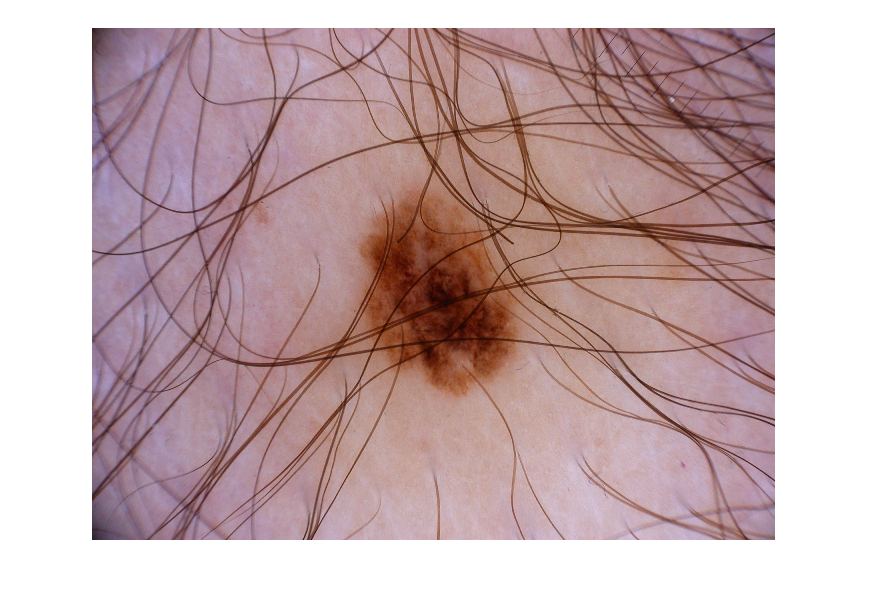
\includegraphics[width=0.45\textwidth]{../results/hair-removal/im_095} 
	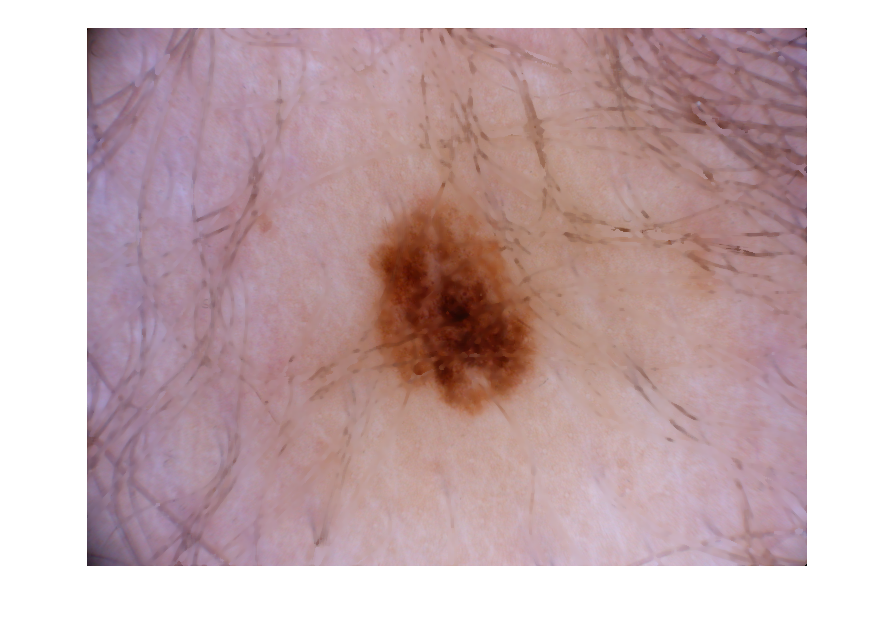
\includegraphics[width=0.45\textwidth]{../results/hair-removal/imshaved_095} \\
	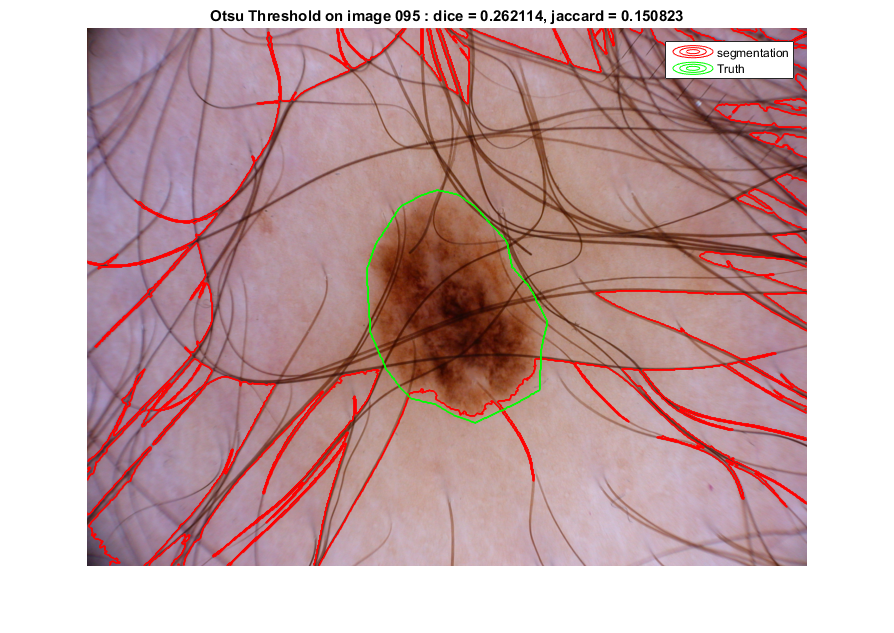
\includegraphics[width=0.45\textwidth]{../results/hair-removal/otsu_segt_im_095} 
	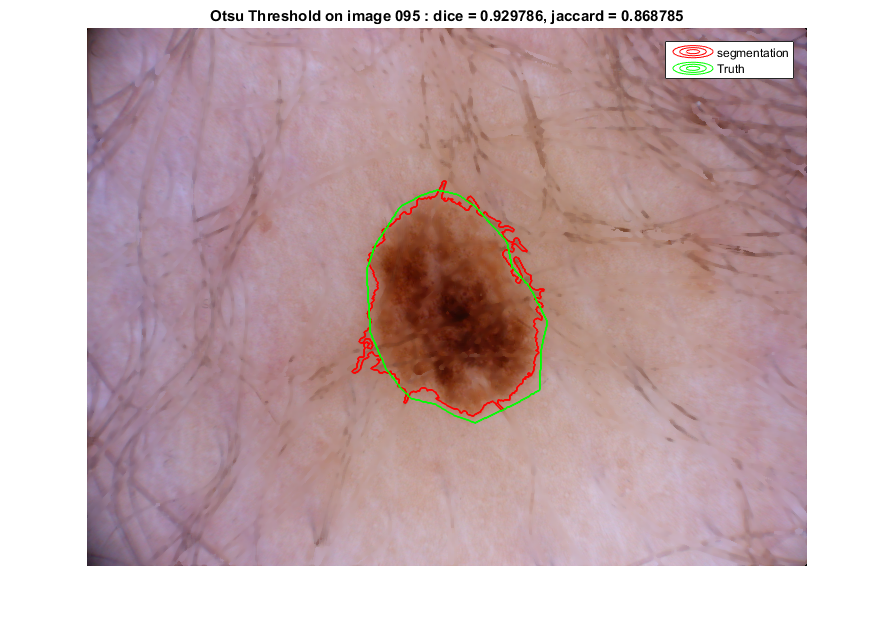
\includegraphics[width=0.45\textwidth]{../results/hair-removal/otsu_segt_shaved_im_095}
	\caption{Importance of hair removal for segmentation}
	\label{fig:dullrazor}
\end{figure}

Example in figure \ref{fig:dullrazor}.

The drawback of this method is all parameters are adapted to be efficient on 512x486 pixels images, whereas the dataset used here contains high resolution images of different sizes (from 720x538 to 2814x2110). The images where therefore resized to the smallest resolution to reduce runtime of the segmentation algorithms and the parameters of the hair removal algorithm were adapted to fit this resolution.

\subsection{Black frame removal}

\begin{figure} 
	\centering
	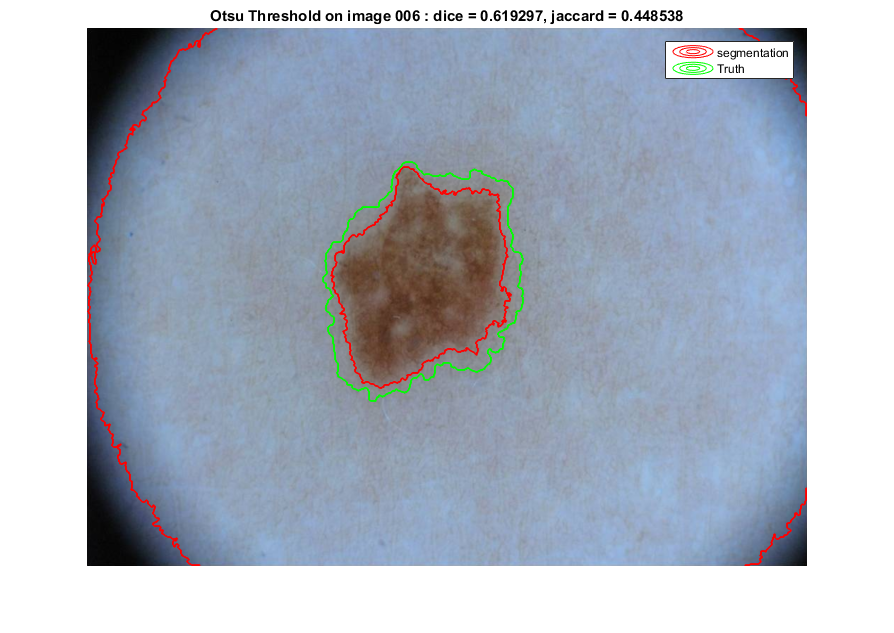
\includegraphics[width=0.45\linewidth]{../results/blackframe/otsu_006_blackframe.png} 
	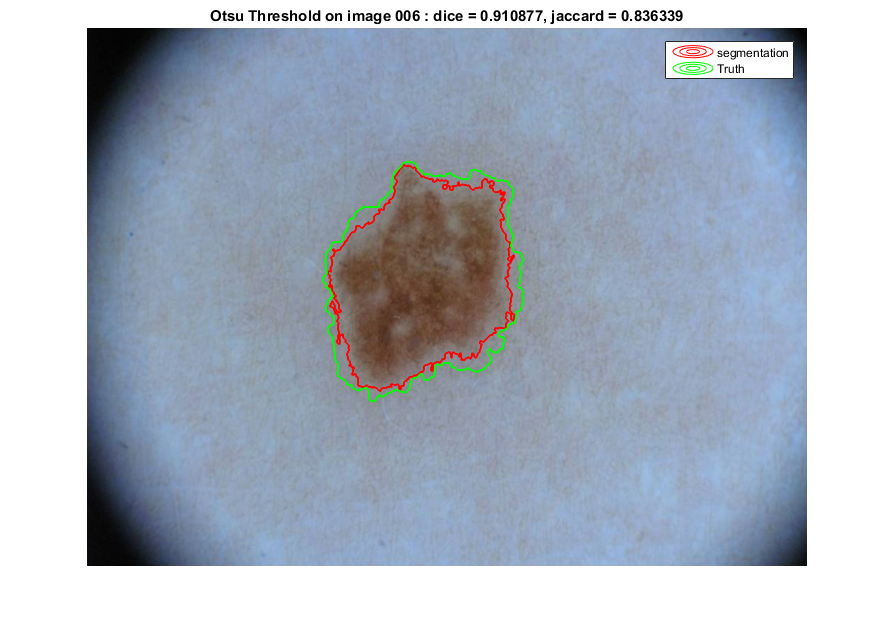
\includegraphics[width=0.45\linewidth]{../results/blackframe/otsu-segt-im-006.png} \\
	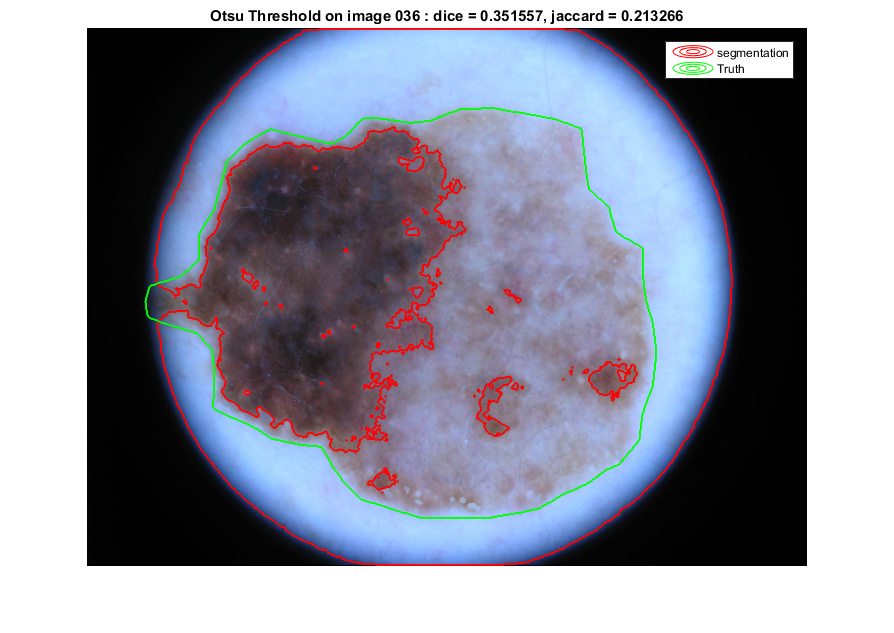
\includegraphics[width=0.5\linewidth]{../results/otsu/otsu-segt-im-036}
	\caption{Importance of black frame removal}
	\label{fig:blackframe}
\end{figure}


We see in figure \ref{fig:blackframe} how the performance increases with the removal of the black frame. Thresholding methods are the most affected since they are non local : the black corner of the image are the darker areas of the image and will therefore be selected as part of the lesion. One way of solving this issue is to perform a connected component analysis and select the ROI among the different clusters in postprocessing. However, this approach is not satisfying because firstly the lesion can be connected to the black frame (figure \ref{fig:blackframe} bottom) and secondly it can have multiple nodules so we can't just keep one "best" region according to any criterion. An additional reason to perform this step in preprocessing for the thresholding methods is to avoid any impact on the selection of the optimal threshold towards the black. We can observe this effect on the two top images of the figure \ref{fig:blackframe} : the ROI expands slightly on the right image. The black frame has been identified before the segmentation process, so that it is not taken into account when choosing the threshold.

\section{Thresholding}
\subsection{Method}
\paragraph{}
Thresholding is the simplest of the 3 methods reviewed here. It takes advantage of the fact that skin lesions are 
usually darker than the surrounding skin. Given a grayscale image, we can 
classify pixels as being part of the region of interest (ROI) or of the 
background based on their intensities. However, using an absolute threshold for all images is not possible because of the color variability. 
\paragraph{} Otsu~\cite{Otsu1979} \tobecompleted{bad phrasing}
gives a way to find an optimal threshold by seeing the histogram as a probability distribution, an choosing the threshold $k^*$ that maximizes the separability measure $\eta$ (equation \ref{eq:eta}) or equivalently the inter-class variance $\sigma_B^2$ because the total variance $\sigma_T^2$ remains constant for any chosen threshold. So the problem comes down to finding the threshold that maximizes $\sigma_B^2$ among the $L$ possible levels of gray as defined in the equation \ref{eq:optimthresh}. 

\begin{equation} \label{eq:eta}
\eta=\frac{\sigma_B^2}{\sigma_T^2} 
\end{equation}
$$
\sigma_B^2=\mathcal{P}(C_0)\mathcal{P}(C_1)(\mu_1-\mu_0)^2
$$
\begin{equation} \label{eq:optimthresh}
  k^* = \argmax_{1<k<L} \sigma_B^2(k)   
\end{equation}

\subsection{Implementation}
- description of the otsu implementation
\tobecompleted{explanation about the implementation}

\subsection{Amelioration}
\paragraph{specific preprocessing:}
The segmentation performance is influence by the color space used. Although~\cite{mendonca_comparison_2007} simply uses the blue channel from RGB color space, but 
Garnavi, Celebi and al~\cite{Garnavi2010} have shown that for a 
threshold-based approach the X channel from CIE-XYZ color space gives better performances. A comparison of the segmentation results can be seen in the figure \ref{fig:color-channel-otsu}

\begin{figure}
	
	\begin{subfigure}{0.7\textwidth}
		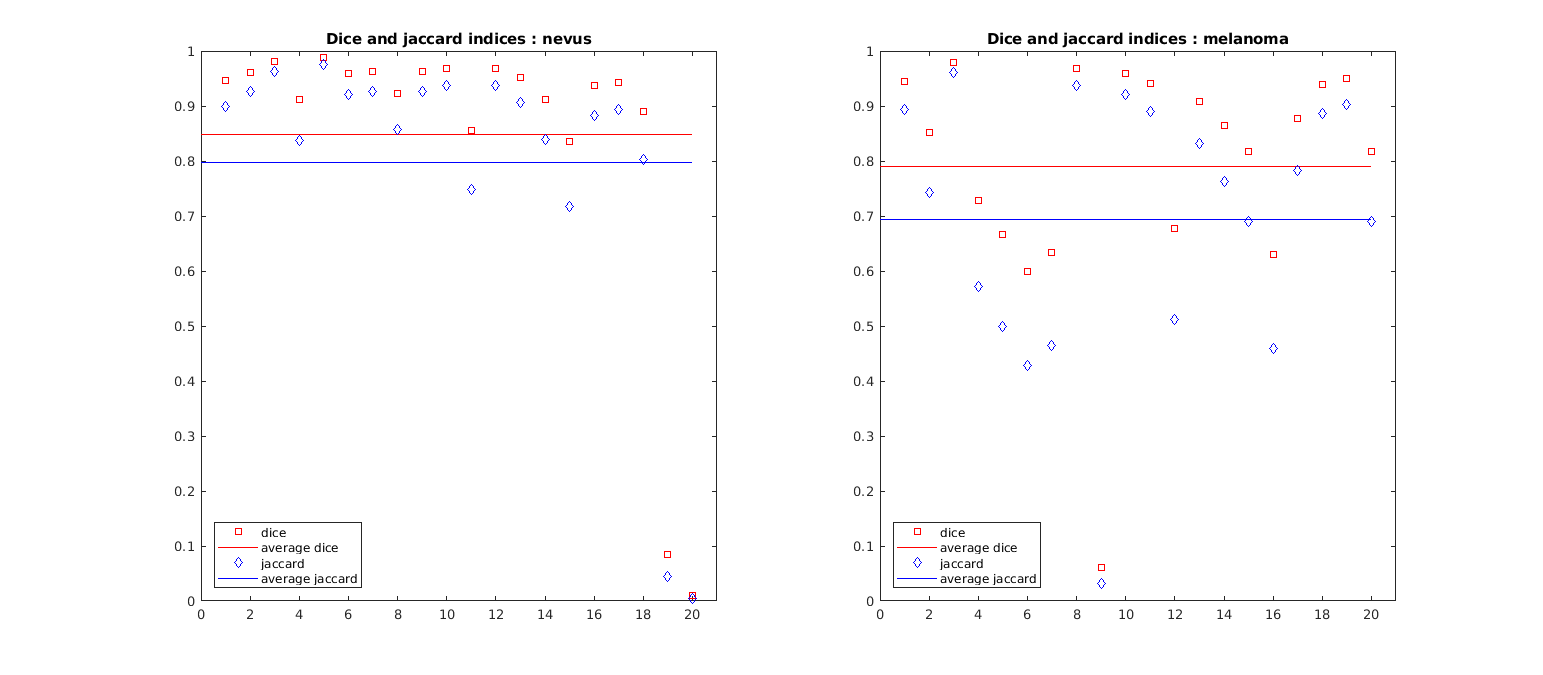
\includegraphics[width=0.9\linewidth]{../results/color-channel-influence/base-evaluation/otsu-dice-jaccard-B.png} 
		\caption{blue channel}
		\label{fig:otsu-blue}
	\end{subfigure}
	\begin{subfigure}{0.7\textwidth}
		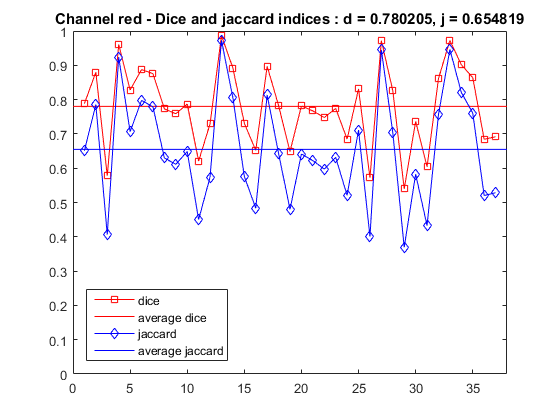
\includegraphics[width=0.9\linewidth]{../results/color-channel-influence/base-evaluation/otsu-dice-jaccard-R.png}
		\caption{red channel}
		\label{fig:otsu-red}
	\end{subfigure}
	\begin{subfigure}{0.7\textwidth}
		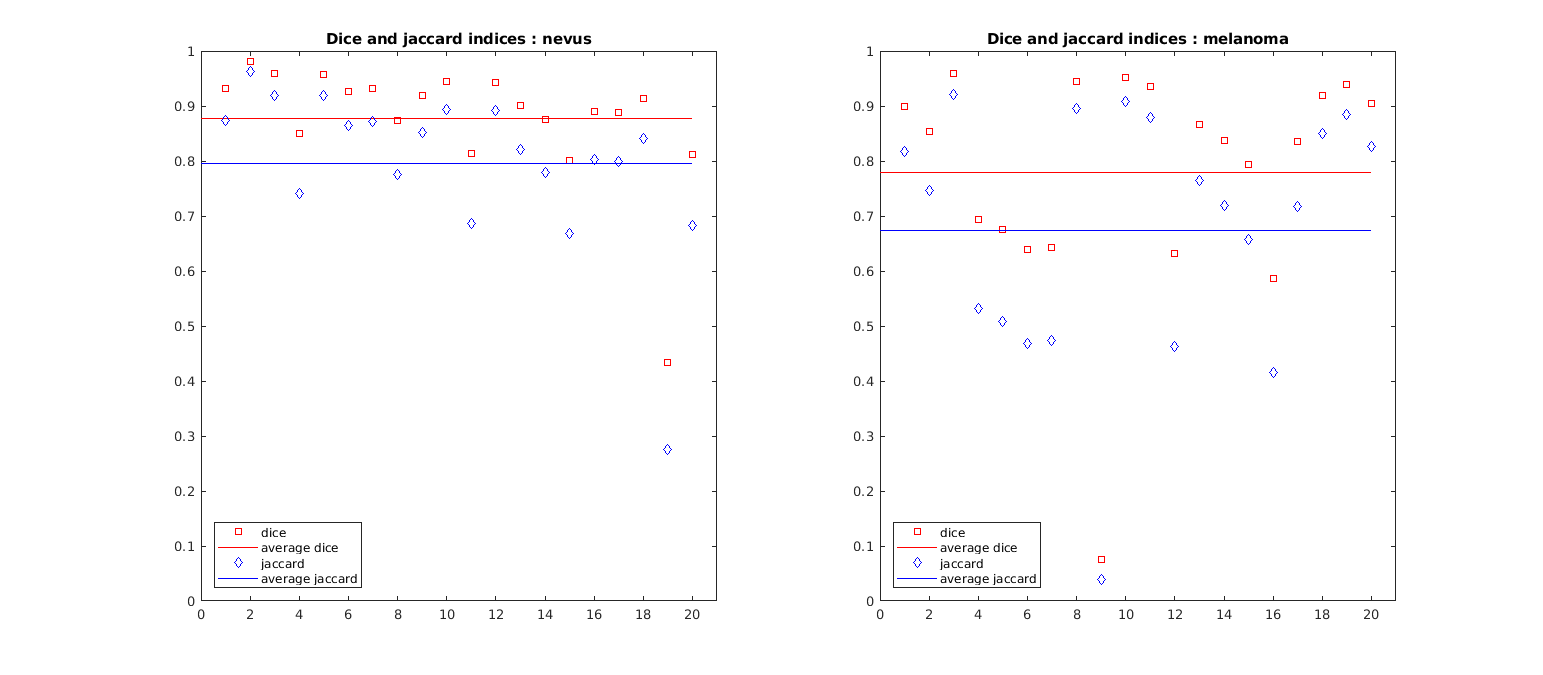
\includegraphics[width=0.9\linewidth]{../results/color-channel-influence/base-evaluation/otsu-dice-jaccard-G.png}
		\caption{green channel}
		\label{fig:otsu-green}
	\end{subfigure}
	\begin{subfigure}{0.7\textwidth}
		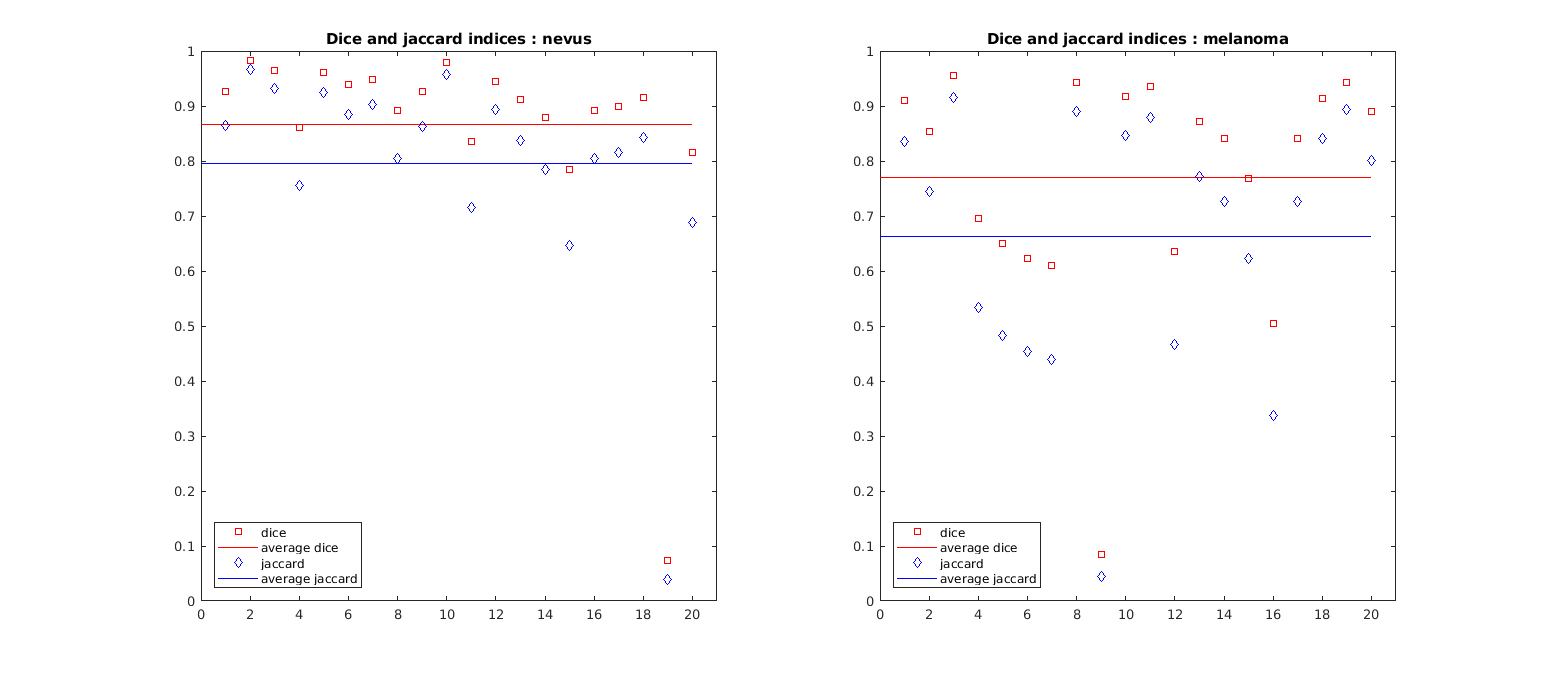
\includegraphics[width=0.9\linewidth]{../results/color-channel-influence/base-evaluation/otsu-dice-jaccard-meanRGB.png}
		\caption{RGB average}
		\label{fig:otsu-mean}
	\end{subfigure}
	\begin{subfigure}{0.7\textwidth}
		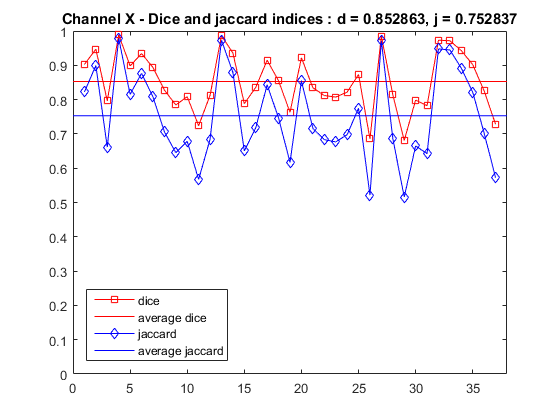
\includegraphics[width=0.9\linewidth]{../results/color-channel-influence/base-evaluation/otsu-dice-jaccard-X.png}
		\caption{channel X from CIE-XYZ}
		\label{fig:otsu-X}
	\end{subfigure}
	
	\caption{Color channel influence on Otsu thresholding performances}
	\label{fig:color-channel-otsu}
\end{figure} \tobecompleted{unclear ! not the best way to show these results... }


\paragraph{specific post-processing:}
- morphological filling
- connected component analysis with several steps (the black border problem)

\subsection{Results}
\tobecompleted{dice and jaccard indices}

dice :
\begin{equation} \label{eq:dice}
d=\frac{2|I \cap J|}{|I| + |J|} 
\end{equation}

jaccard :
\begin{equation} \label{eq:jaccard}
j=\frac{|I \cap J|}{|I \cup J|} 
\end{equation}

\section{Region based segmentation}
\subsection{Method}
First, a simple region growing algorithm, but to slow and bad performances so SRM was used
\paragraph{} Statistical Region Merging~\cite{nock_statistical_2004} has been 
used by Celebi and al~\cite{celebi_border_2008} to perform a fast and efficient 
segmentation of skin lesions. This approach consists in merging regions in a particular order, with a statistical criterion.

$$
f(p,p')=|p-p')
$$
\subsection{Implementation}

\subsection{Results}
dice, jaccard, etc, weak and strong aspects, etc

what would it take to make it fullly auto ?

\section{Parametric active contours}
\subsection{Method}
\paragraph{}  Distance Regularized Level Set Evolution \cite{li2010distance} \tobecompleted{method description}
\subsection{Implementation}
Very sensitive to the initialization of the contour, and to the parameters: hard to tune.

\subsection{Results}

BLABLA dice, jaccard etc
blabla

What would it take to make this method fully auto ?

\section{Comparison}

\subsection{Perfomances}
- dice, jaccards, etc
- runtime
- what are the problems for each
- sensitive to init for the semi auto ?
- etc : PUT PERFORMANCE DATA ABOUT THE DIFFERENT METHODS
ETC

\subsection{Choosing the right method}
An interesting development of this comparison would be to have a efficient and easily computable criterion to choose the best method given a particular image. Of course this would make more sense if all the methods were fully automated, since here an interaction with the user is already needed, we can compute the three methods and give a choice. But as we have seen, it is possible to avoid this interaction given some further development, and it has been done in the literature for the SRM method~\cite{celebi_border_2008}. 

\subsubsection{Separability criterion}
To compute the threshold with Otsu's method, we optimize a separability measure $eta$. We investigated whether there were a correlation between this value and the evaluation metrics, so that it could be used to evaluate the performance of the thresholding algorithm. The results are shown in figure \ref{fig:eta-correlation} and it appears that $\eta$ does not make a good selection criterion, for several reasons. Even in the case of critical failure, it still has a high value. That is because $\eta$ is measuring the inter-class variance normalize by the total variance, but two very contrasted class are not a guarantee for a good performance. The difficult images often show a lesion with a high inner-class variance that are separated by the thresholding method without deteriorating the value of $\eta$.

Another approach for using the separability measure would be to use not only the value associated with the optimal threshold but the entire set associated with all possible thresholds. The evolution of this measure could give us knowledge about Otsu's algorithm performance.

\subsubsection{another criterion}

\begin{figure}
\centering
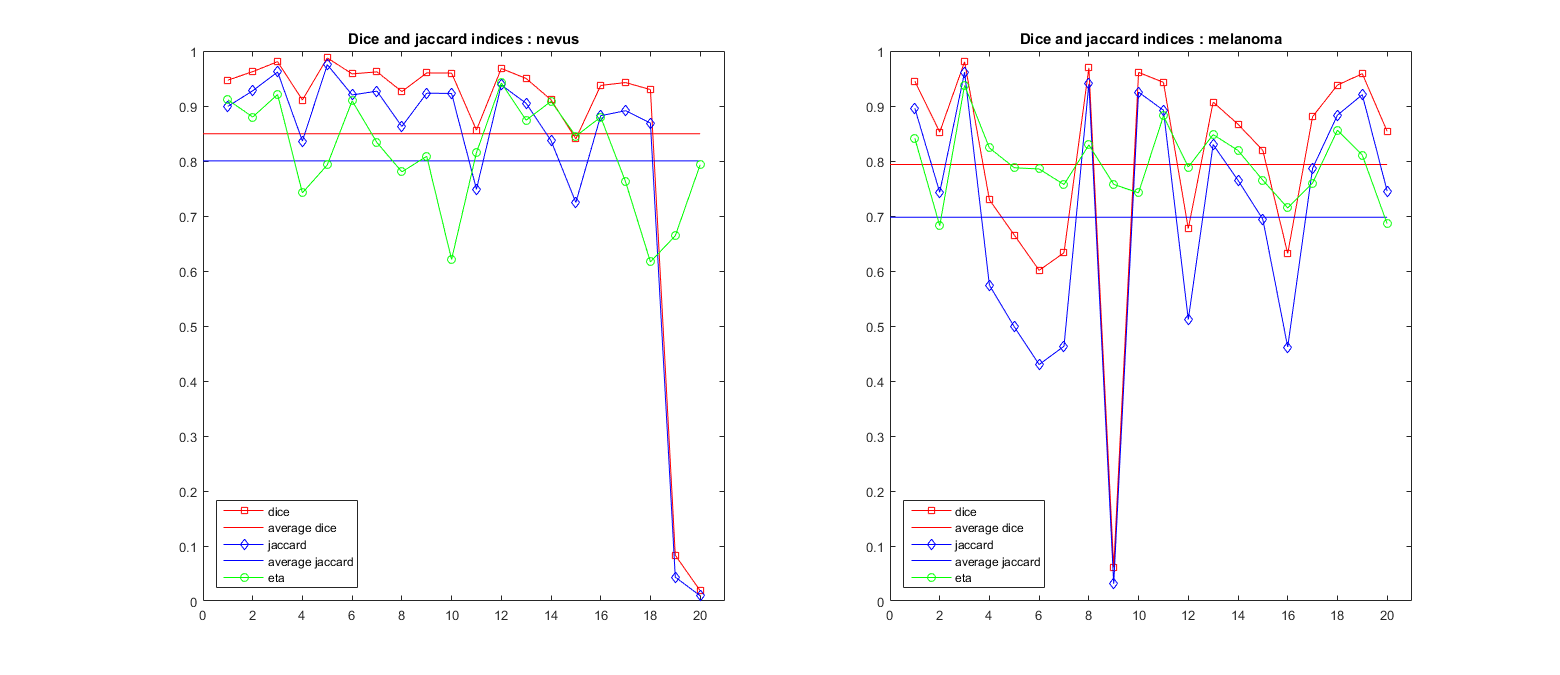
\includegraphics[width=0.9\linewidth]{../results/otsu-dice-jaccard-eta-plot}
\caption{$\eta$ (green), dice (red) and jaccard (blue) indices.\\ Correlation coefficient : R($\eta$, dice)=0.33, R($\eta$, jaccard)=0.37 }
\label{fig:eta-correlation}
\end{figure}


\section*{Conclusion}
%TODO Conclusion
 Quality of groundtruth : difficult to have a gold standard because of fuzzy borders, etc... here there was a problem because 2 methods of Manual segmentation were used. Also : only one segmentation mask was available, so we can not compare our result with the inter-expert variability.

 Complementarity of the different methods
 automatic criterion to decide between the different methods ? (examples : otsu's separability measure does not work, presence of hair, global initial contrast, etc... complicated...)
 
 Preprocessing is critical
 
discuss quality of the method used



\bibliographystyle{plain}
\bibliography{PRIM-rapport}

\end{document}
